\subsection{Approval, Execution, and Evidence}
\label{sec:routes}
\label{sec:mech}
\label{sec:objective}
\label{sec:nodeexec}
\label{sec:ack}
\label{sec:agentloop}
Routes add timing and approval checks appropriate to their operation. Online
node writes enforce a 60\,s minimum spacing; recipe trials use a per-line
cadence (300\,s by default), and recipe intervals are anchored to approval.
Manual approval binds an actor and proposed operation to candidate values,
applicable limits, expiry, and the active line--product--recipe--run tuple.
After approval, the handler rechecks authority and compares the current tuple
with the approved tuple before entering DCW dispatch. The default approval
wait expires after 180\,s. A changed recipe definition requires a new
\texttt{recipe\_apply} proposal. These checks reject stale requests at the
software dispatch boundary; they do not lock equipment state across network
or device I/O.

Fig.~\ref{fig:hitl}(a) illustrates the four-layer value interval in
Eq.~(\ref{eq:admission}) using an illustrative RPM configuration. Panel (b)
shows a symbolic approval followed by authority and context rechecks; its
values are illustrative, not experimental measurements.

\begin{figure*}[!t]
\centering
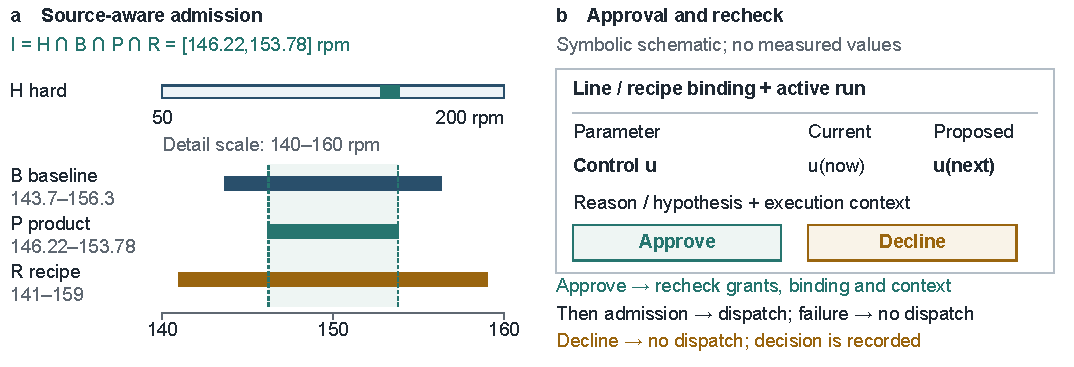
\includegraphics[width=\textwidth]{resources/fig-admission-hitl-2026.pdf}
\caption{Admission and approval boundaries. (a) Illustrative RPM
configuration, not experimental data: online node interventions use the
four-layer interval of Eq.~(\ref{eq:admission}), whereas recipe dispatch
omits the previous recipe window. (b) Symbolic human approval binds a
proposed action and its context tuple; execution rechecks the active
line--product--recipe--run context, authority, and applicable limits.
Approval does not reserve equipment state.}
\label{fig:hitl}
\end{figure*}

A \texttt{recipe\_trial} illustrates the operation sequence: the handler
checks the bound recipe, active run, candidate parameters, and route timing;
if required, it requests approval; after revalidation, it submits a bounded
batch through the configured driver and returns a per-parameter receipt.
The caller obtains later DAQ observations separately and may then update,
apply, or roll back a recipe. A trial neither saves nor applies a recipe
version. The driver registry maps semantic controls to configured protocol
drivers, keeping protocol details out of agent operation arguments.

Receipts and observations answer different questions. A command result is
graded as readback-verified, transport-acknowledged, or unverified; a
readback mismatch can trigger up to three reads at 2\,s intervals. Recipe
batches retain per-parameter verification outcomes. DAQ stores subsequent
timestamped process observations, while recipe versions, approvals, and
task records remain service-owned records linked where a route supplies the
corresponding identifiers. A verified setpoint confirms the command path,
not target attainment. This distinction defines the evidence chain evaluated
in Section~\ref{sec:eval}.
